\documentclass[10pt,conference,compsocconf]{IEEEtran}

%\usepackage{times}
%\usepackage{balance}
\usepackage{url}
\usepackage{graphicx}	% For figure environment
\usepackage{siunitx}
\sisetup{
  range-phrase = \ {,}\ ,
  range-units  = brackets,
  open-bracket = [,
  close-bracket= ],
}

\usepackage{booktabs}
\usepackage{amsmath,amssymb}
\usepackage{xcolor}
\newcommand\TODO[1]{\textcolor{red}{#1}} % for all TODOs
\usepackage{pdfpages}

\begin{document}
\title{Deep Generative Models for High-Resolution Cosmology Images}

\author{Till Schnabel, Sven Kellenberger, Hannes Pfammatter, Michelle Woon \\Group: Galaxy Crusaders, Department of Computer Science, ETH Zurich, Switzerland}

\maketitle

\begin{abstract}
This paper explores various machine learning models for generating sparse, high-resolution cosmology images. %We describe these models and our motivation for their usage.
%These models are described and the motivation for their usage is explained. 
The contribution of this paper is twofold. Beside the design of models for cosmology image generation, a similarity function, which is part of our data, is learned.

The generative models are compared to a simple baseline model and evaluated by estimating the values of the similarity function. We found that extracting the most important features from the images and designing generative models for these features only produced the best results. Our approximation of the similarity function achieved $2^{nd}$ place on both the public and private test data set.
%$2^{nd}$ best result on both public and private Kaggle test data sets.


%This paper explores various ways for generating as well as approximating a similarity function for high resolution cosmology images. The methods solving the latter issue is evaluated via Kaggle\cite{Kaggle}, achieving 2nd place on the public leaderboard.

%For the similarity score approximator, an advanced Random Forest (RF) method is evaluated and compared to a Convolutional Neural Network (CNN) and a simpler RF approach. The structure of our CNN will be introduced and analyzed. This paper also provides insights to the advanced RF used, such as how and why it performed better than the CNN. We will also discuss the image preprocessing and data augmentation used for all learning methods introduced in this paper. 

%For the generation of the highly space cosmology images, an adhoc method, a Variational Autoencoder (VAE), a conditional Deep Convolutional Generative Adversarial Network (cDCGAN) and also a PixelCNN \TODO{(leave this?)} approach are all explored. We will discuss and evaluate each method in this paper. We present our cDCGAN on k-means clustered stars method.
\end{abstract}

\section{Introduction}
\label{sec:introduction}
Generative modeling is not a new area of research. However, with the recent advent of deep generative models the research interest in this area has increased drastically. 

In this project, we study the generation of cosmology images. Our cosmology images are sparse, high-dimensional data, which has proven to be an interesting problem suitable for the application of mathematical methods and machine learning models.

We split our project into two parts. First, we designed multiple machine learning models for cosmology image generation. Our starting point was a deep convolutional generative adversarial network (DCGAN) capable of generating cosmology images with high resolution. As this model was not able to capture important features such as stars with enough detail, we decided to focus on generating these features only for the other models. 
For the generation of stars only we designed a variational autoencoder (VAE), a DCGAN and used an existing PixelCNN. 
Our final solution consists of a conditional DCGAN (cDCGAN) that is able to generate several classes of stars that were found by clustering.

Second, we designed a convolutional neural network (CNN) and used an off-the-shelf random forest (RF) regression model to learn the similarity function which is part of our data. Finally, we evaluated our generative models by estimating the similarity scores of the generated images. 

%Our data set consists of \SI{1200}{} labeled images with labels indicating whether an image is a cosmology image or not and \SI{9600}{} scored images with scores indicating the similarity of an image to the prototypical cosmology image. We refer to them as labeled images and scored images.

%%%%%%%%% TODO
%\TODO{Mention the best generator. (cDCGAN?)}
%%%%%%%%%

%\TODO{Related work is not in the guideline, but I guess they add them in "Models and Methods"}
%\section{Related Work}
%To prevent overfitting, Srivastava et al.\@ \cite{Dropout} introduced Dropout in 2014. The idea is that e.g.\@ a fully connected layer is followed by such a dropout layer that sets a configurable percentage of output neurons to zero during training, thus effectively omitting their impact on the final output. Consequently, the preceding layer is less likely to overfit to training data, because it is forced to learn a more meaningful representation of the data using all neurons.

%In 2015, Ioffe et al.\@ \cite{BatchNorm} introduced BatchNorm --- a normalization technique that takes as input the batch of data and normalizes across this batch. Other than for instance normalization during pre-processing, a BatchNorm layer contains learnable mean and variance, s.t.\@ the network may adjust to covariate shifts and vanishing gradients in between layers. Today, it is widely used in classification and other networks, to speed up the learning process.

%Also in 2015, He et al.\@ \cite{ResNet} released their ResNet architecture, which uses so-called ``Skip connections'' that allow for far deeper architectures than practical ones before. The output of a building block of a few convolutional layers is summed with this block's original input, which allows the network to skip unwanted blocks. This process, they call ``Residual learning''. The problems of deep architectures like zero gradients were compensated by this new invention.

\section{Models and Methods} \label{sec:models_methods}
%This section briefly describes the models and methods which were used for this project and explains the motivation for their usage. 
The data set used for this paper was obtained from Kaggle. It consists of labeled images ($\in \{0,1\}$ depending if it is a cosmology image or not), scored images (based on their similarity) and query images (to be scored and uploaded to Kaggle).

We built all our neural networks using the Keras (Chollet et al.\@ \cite{chollet2015keras}) API on the TensorFlow (Abadi et al.\@ \cite{tensorflow2015-whitepaper}) backend and trained them on a single NVIDIA Tesla V100-SXM2 \SI{32}{GB} GPU on the Leonhard Cluster.

\subsection{Approximation of the Similarity Function}

\subsubsection{Random forest regression baseline} 
Random forests were introduced in 1995 by Ho \cite{Ho} and further developed in 1999 by Breiman \cite{Breiman}. In this work, they were used as an off-the-shelf model for regression. By improving on this baseline we also achieved our best result for approximating the similarity function. 

For training, histograms of image properties were used as input features. We started with a histogram of pixel intensities which we consider as our baseline model. In 2007, Bosch et al.\@ \cite{Bosch} used random forests for image classification. They captured information on shape by computing histograms of oriented gradients (HOG) of edges inside image regions. We computed a similar histogram for the entire image and combined it with the histogram of pixel intensities, which improved the accuracy of the regression.

What worked best was a histogram of the power spectrum of the images. To capture the power spectrum in a histogram, we used the fast Fourier transform (FFT) and applied a log transformation. Lastly, we searched for regions of interest (ROIs) by filtering out high frequencies, low frequencies or certain orientations.
%We added histograms of regions of interest (ROI) where we filtered out low frequencies, high frequencies or certain orientations, but were not able to substantially improve the results.

%\subsubsection{CNN} % hard baseline
%For the neural network approach for image classification, we used a deep convolutional architecture. We experimented a lot with the specific layers. Most experiments were performed on lower-resolution images ($125\times125$ and $250\times250$), because simple patterns like the star distribution could similarly be captured on this resolution while saving lots of computation time. Good settings were then applied to the original data. Our most important discoveries were:
%\begin{itemize}
%    \item Batch normalization (Ioffe and Szegedy \cite{BatchNorm}) greatly stabilizes and thus accelerates the training.
%    \item Because the final score is linear between 0 and 8, a sigmoid layer times 8 in the end makes it harder for the network to predict the score correctly and is thus counter beneficial.
%    \item A fast fourier transform (FFT) preprocessing improves and stabilizes the training.
%    \item Many convolutions but few parameters lead to the best results, because more convolutions mean a greater receptive field and a lot of parameters quickly cause overfitting on the sparse images.
%    \item We did not find residual connections (He et al.\@ \cite{ResNet}) to be helpful.
%    \item Dropout (Srivastava et al.\@ \cite{Dropout}) reliably prevents the network from early overfitting.
%\end{itemize}
%Our final architecture can be seen in figure \ref{fig:nn_classifier_arch}.  Not mentioned is the padder that pads the intermediate code from $125\times125$ to $128\times128$ spatial resolution. The number of features were raised by a factor of 2 every stacked convolutional block (colored in blue) until the maximum of 32 was reached. In total, there were eight of these blocks. No bias was used. The network had a total of only \SI{37376} parameters, \SI{37120} of which trainable. As mentioned, the images were preprocessed with FFT. During training, the data were augmented with horizontally and vertically flipped with a probability of \SI{0.5} as well as randomly shifted in height and width by up to \SI{20}{\percent}. We reached a score of \SI{0.16792} on the public and \SI{0.18781} on the private part of the test set, after training the model for 140 epochs.

\subsubsection{CNN baseline} % hard baseline
We used a convolutional neural network (CNN) with a deep architecture (see for instance LeCun et al.\@ \cite{DeepLearning}) as our second model for approximating the similarity function. To speed up computations, we performed most experiments on images with dimensions $\SI{125}{}\times\SI{125}{}$ and $\SI{250}{}\times\SI{250}{}$. We experimented with convolution depth, normalization (see Ioffe and Szegedy \cite{BatchNorm} for BatchNorm), number of features, residual connections (He et al.\@ \cite{ResNet}), preprocessing and augmentation.
%\begin{itemize}
%\item Batch normalization (Ioffe and Szegedy \cite{BatchNorm}) stabilized and accelerated training.
%\item A scaled sigmoid activation function at the output of the network deteriorated accuracy.
%\item Raising the number of convolutions increased the receptive field and thus improved accuracy.
%\item Due to the sparsity of the images, fewer parameters prevented the network from overfitting.
%\item We did not find residual connections (He et al.\@ \cite{ResNet}) to be beneficial.
%\item Dropout (Srivastava et al.\@ \cite{Dropout}) prevented the network from early overfitting.
%\item Using the log-transformed power spectrum of the images as input to the network improved accuracy.
%\end{itemize}
Our final architecture is shown in Figure \ref{fig:nn_classifier_arch}. The network contains a total amount of \SI{228680}{} trainable parameters. The images are all preprocessed with the log-transformed power spectrum. For training, we augmented the data using horizontal and vertical flips with probability \SI{0.5}{} as well as random shifts in height and width by up to \SI{20}{\percent}. The model was trained for \SI{140}{} epochs. % epochs in Results?

\begin{figure}
    \centering
    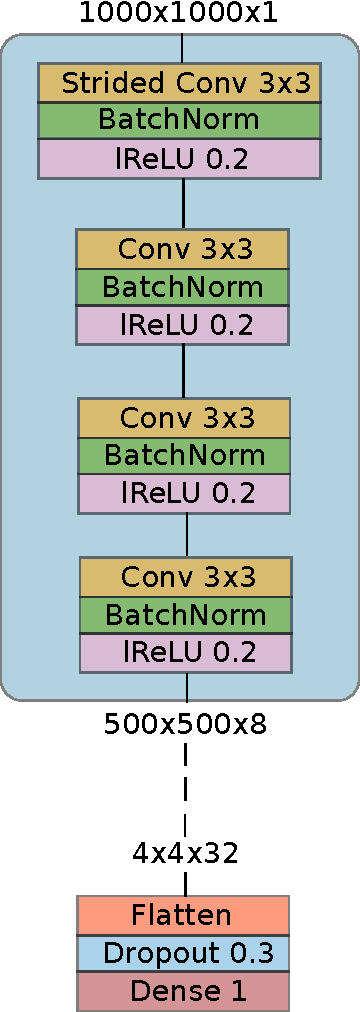
\includegraphics[width=0.35\columnwidth]{assets/nn_classifier_arch.pdf}
    \caption{Illustration of the CNN architecture. ``(Strided) Conv 3x3'' denotes a convolutional layer with a $\SI{3}{}\times\SI{3}{}$ kernel; the stride is \SI{2}{} for ``Strided Conv'' and \SI{1}{} for the rest.
    The input is an image of dimension $\SI{1000}{}\times\SI{1000}{}\times1$. The spatial resolution is reduced by a factor of \SI{2}{} in height and width per stacked convolutoinal block (colored in blue), of which there are 8 in total. The padding layer used for mapping the spatial resolution from $\SI{125}{}\times\SI{125}{}$ to $\SI{128}{}\times\SI{128}{}$ is omitted. The number of feature maps increases by a factor of \SI{2}{} with each block until \SI{32}{} is reached. ``Dense 1'' outputs the final $1$-dimensional prediction score.} % lReLU, BatchNorm, Dropout and Flatten should be self-explanatory 
    \label{fig:nn_classifier_arch}
\end{figure}

%\subsubsection{CNN} % hard baseline
%We used a convolutional neural network (CNN) with a deep architecture as our second model for approximating the similarity function. In this subsection, the architecture of the CNN is introduced and analyzed.
%To speed up computations, most experiments were performed on images with dimensions $\SI{125}{}\times\SI{125}{}$ and $\SI{250}{}\times\SI{250}{}$. Our most important findings were:

%\begin{itemize}
%\item Batch normalization (Ioffe and Szegedy \cite{BatchNorm}) stabilized and accelerated training.
%\item A scaled sigmoid activation function at the output of the network deteriorated accuracy.
%\item Raising the number of convolutions increased the receptive field and thus improved accuracy.
%\item Due to the sparsity of the images, fewer parameters prevented the network from overfitting.
%\item We did not find residual connections (He et al.\@ \cite{ResNet}) to be beneficial.
%\item Dropout (Srivastava et al.\@ \cite{Dropout}) prevented the network from early overfitting.
%\item Using the log-transformed power spectrum of the images as input to the network improved accuracy
%\end{itemize}

%Based on these findings, our final architecture is shown in figure \ref{fig:nn_classifier_arch}. It consists of 8 stacked convolutional blocks where only the first one is shown in figure \ref{fig:nn_classifier_arch}. The number of feature maps is increased by a factor of 2 in each stacked convolutional block until a maximum amount of \SI{32}{} feature maps is reached. The padding layer used for mapping the spatial resolution from $\SI{125}{}\times\SI{125}{}$ to $\SI{128}{}\times\SI{128}{}$ is omitted. The network contains a total amount of \SI{228680}{} trainable parameters.
%For training, we augmented the data using horizontal and vertical flips with probability \SI{0.5}{} as well as random shifts in height and width by up to \SI{20}{\percent}. The model was trained for \SI{140}{} epochs. We achieved mean absolute errors (MAE) of \SI{0.168}{} and \SI{0.188}{} on the public and on the private Kaggle test data set.



\subsection{Cosmology Image Generation}

\subsubsection{Adhoc Generator (AG) baseline} % easy baseline
Cosmology images in the given data sets are, in essence, white stars on a black background, as such we were able to use a simple tiling method for our easy baseline. This is done by copying stars from the available data and placing them onto a black background. Using the available labeled data, we detect stars in all the cosmology images by finding contours in the image. Doing this also allows us to find the minimum and maximum amount of stars in a cosmology image.

Each image to generate first starts out as a black destination image. Then, for each image to generate, a random number between the minimum and maximum amount of stars is selected. For each star to place into the image, a random source cosmology image is chosen and then a random star from that source image is taken. That star is then placed on a random spot in the destination image.

\subsubsection{Large DCGAN}

\begin{figure}%[ht]
    \centering
    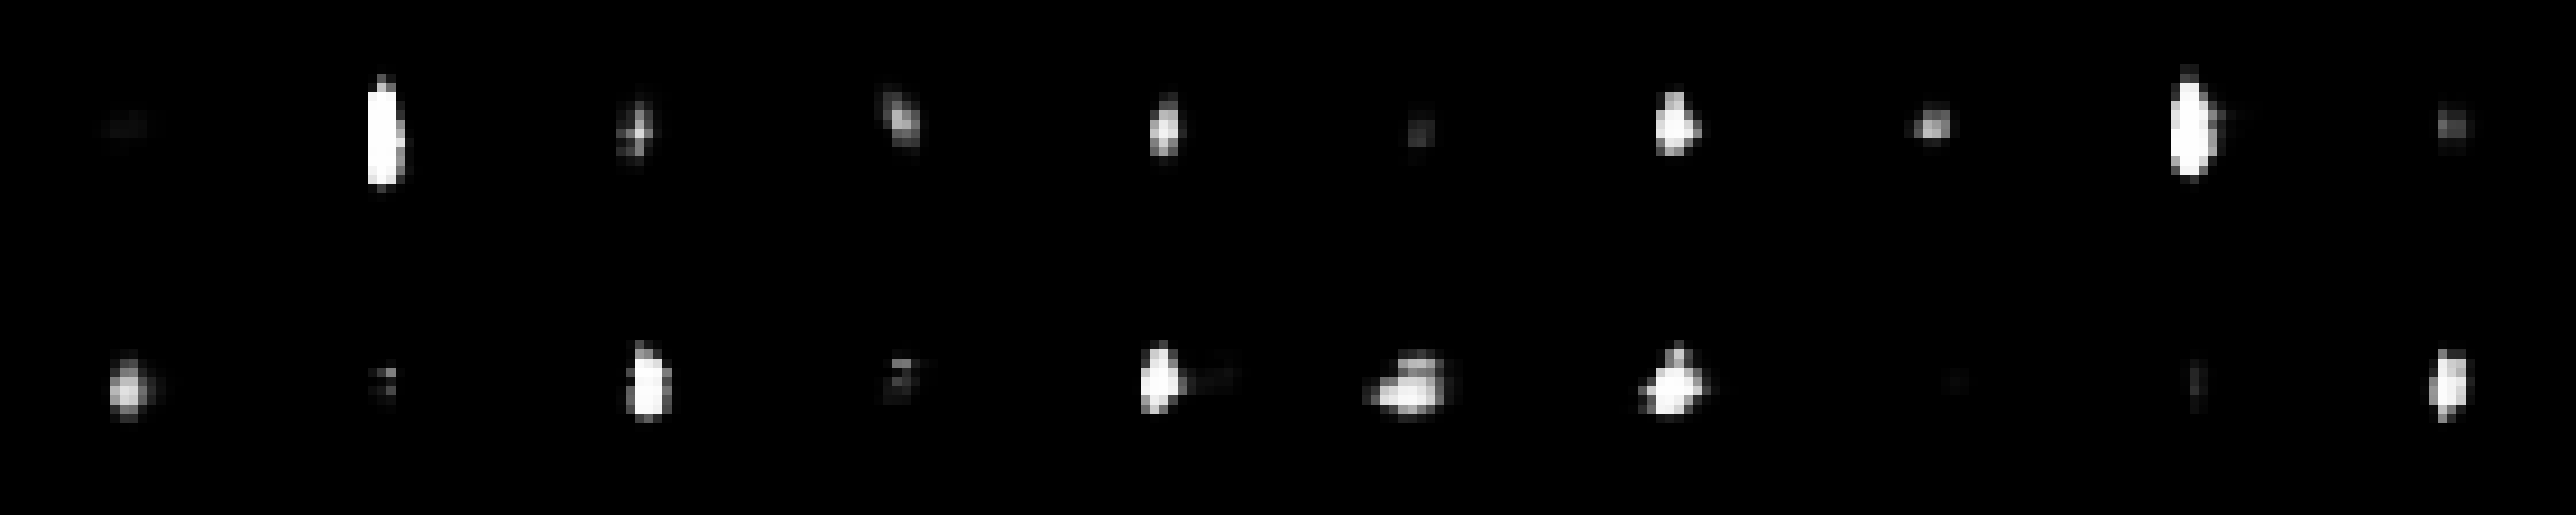
\includegraphics[width=\columnwidth]{assets/star_ensemble_large_resized.png}
    \caption{Random selection of stars generated by the large DCGAN.}
    \label{fig:dcgan_stars}
\end{figure}

The deep convolutional generative adversarial network (DCGAN) was introduced in 2015 by Radford et al.\@ \cite{Radford}. It is a generative adversarial network (GAN) where both generator and discriminator are convolutional neural networks (CNNs) with architectural constraints which stabilize training. We used a large DCGAN to generate entire cosmology images. 

Our implementation is based on on a reference implementation on the TensorFlow website \cite{dcgantf} as well as on the original paper and implementation. As proposed by Odena et al.\@ \cite{Odena} we used nearest neighbor interpolation and convolution instead of transposed convolution.

For training, all labeled images and all scored images in the data set with similarity score greater or equal to \SI{2.61}{} were used. The pixel intensities were normalized to the range \SIrange{-1}{1}{} and the images were padded to dimensions $\SI{1024}{}\times\SI{1024}{}$ to simplify upsampling and strided convolutions. Generator and discriminator contain a total amount of \SI{6491125}{} trainable parameters.

\subsubsection{VAE on stars} % hard baseline
In our second approach, we focused on the generation of the most important features only. We used a variational autoencoder (VAE) to generate images of stars and placed them within a black background. 

The VAE was introduced in 2014 by Kingma and Welling \cite{DBLP:journals/corr/KingmaW13}. It allows the encoding of data points to low-dimensional latent representations  $\sim\mathcal{N}(0, I)$ and to generate new data points by decoding arbitrary latent vectors $\sim\mathcal{N}(0, I)$. This is achieved by learning to map each data point $x$ to a Gaussian distribution $q_{\phi}(z|x)$ determined by $\mu$ and $\sigma$ and each latent vector $z$ to a Bernoulli distribution $p_{\theta}(x|z)$ determined by $p$.
 
Our implementation is based on the original paper as well as on the tutorial on variational autoencoders by Doersch \cite{doersch2016tutorial} and on a reference implementation on the TensorFlow website \cite{cvaetf}. Because stars are shaped in a similar fashion, a multilayer perceptron (MLP) with a single hidden layer of size \SI{500}{} is used for both the probabilistic encoder $q_{\phi}(z|x)$ and the probabilistic decoder $p_{\theta}(x|z)$. The parameters of the MLPs are denoted by $\phi$ and $\theta$. The latent dimension is set to \SI{16}{}. 

For training, only the labeled images were used. Using the approach of the adhoc generator, stars were extracted and centered inside images of size \SI{28}{}x\SI{28}{}. The pixel intensities were normalized to the range \SIrange{0}{1}{}. The MLPs contain a total amount of \SI{811816}{} trainable parameters. To create cosmology images, generated star images were distributed randomly inside an image with black background. The number of stars per image is normally distributed and estimated from the labeled images. 


\begin{figure}
    \centering
    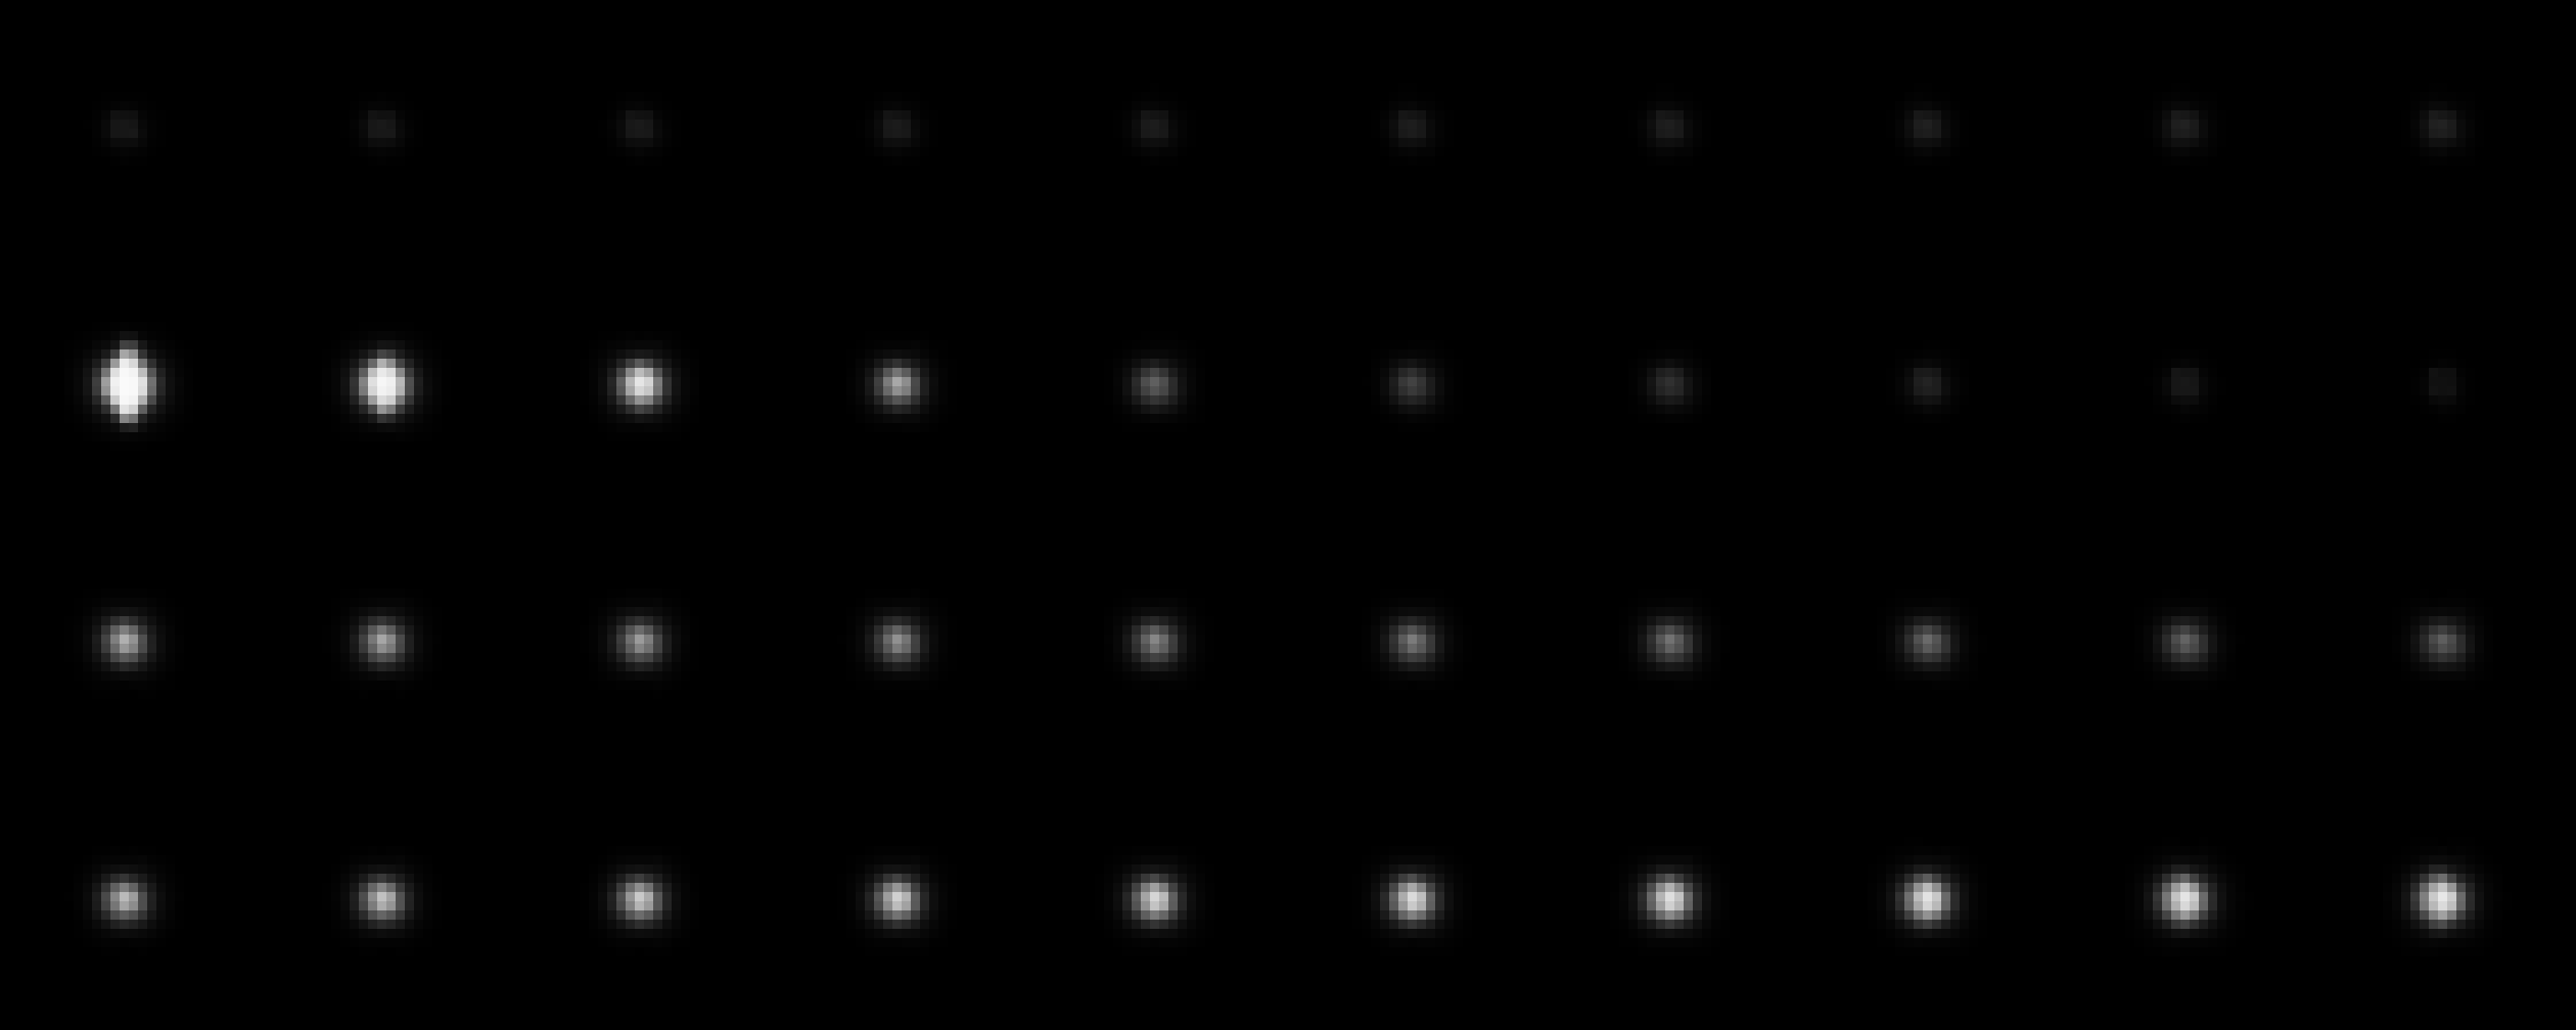
\includegraphics[width=\columnwidth]{assets/vae_interpolation_resized.png}
    \caption{Linear interpolation between vectors in the latent space of the variational autoencoder on stars.}
    \label{fig:vae_interpolation}
\end{figure}

\subsubsection{cDCGAN on stars}
Taking the same approach as with the VAE, we also trained a smaller DCGAN on our data set of extracted stars.
In order to control the star distribution in an image more precisely, we decided to cluster the star images. Considering our large data set of about \SI{15000}{} star images, most of them looked very similar, which is why we chose to divide them into five distinct classes. To achieve that, we trained a simple deep convolutional autoencoder (DCAE) on the star images for 400 epochs and applied $k$-means clustering on each image's latent code. We did not have to worry about overfitting the DCAE, because it was only used on the data it was trained on.

Afterwards, we used the clustered data to train a conditional DCGAN (cDCGAN). Beside the image/latent code, the generator/discriminator was also fed the class label belonging to a star. In order to find a good distribution for the final images, we measured the number of occurrences of each star class per cosmology image and approximated it with a normal distribution bound to unsigned integers. We assumed the positioning of a star to be distributed uniformly. We then placed the stars generated by the cDCGAN into \SI{100}{} background images and repeated this process for \SI{2000}{} times to find those random numbers that produced the highest mean similarity scores (MSS) as estimated by our random forest (RF) and CNN models. We included this deterministic image stitching and MSS estimation as validation score into the training of our final cDCGAN.


The architecture of the cDCGAN was adopted from the reference implementation on the TensorFlow website \cite{dcgantf}. No adjustments to the resolution had to be made, only the conditional property had to be added. The architecture of the conditional generator is shown in Figure \ref{fig:cgen_arch}. It uses a total amount of \SI{3212480}{} trainable parameters. Figure \ref{fig:clustered_generated_stars} shows generated samples of the five different star classes. The discriminator uses \SI{269313}{} trainable parameters. Its architecture is illustrated in Figure \ref{fig:cdis_arch}. The total amount of parameters is high compared to e.g.@ the CNN and could have been reduced. However, since the generation of such small images is very stable, no architectural experiments were conducted. The cDCGAN was trained for 185 epochs, and about half the training time was spent on validation.

\begin{figure}
    \centering
    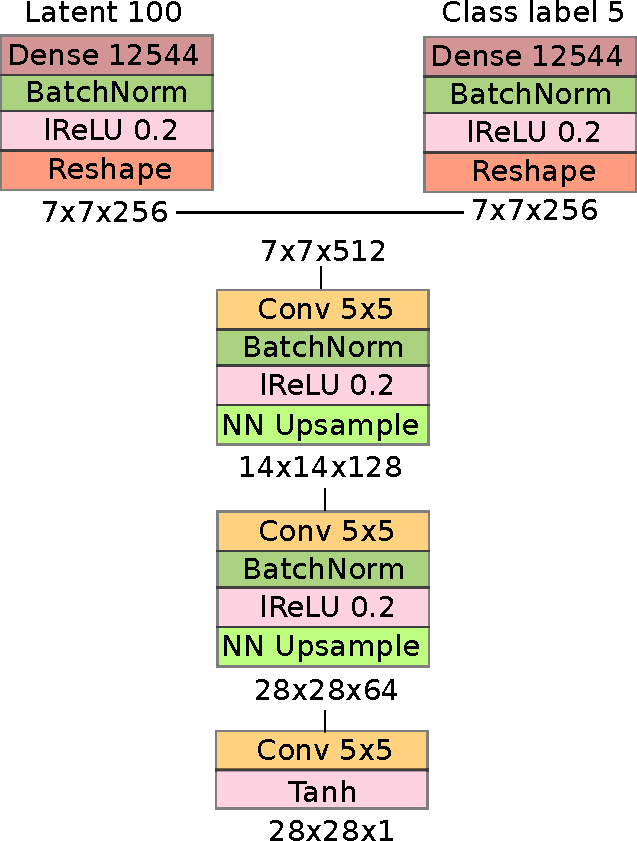
\includegraphics[width=0.58\columnwidth]{assets/cgen_arch.pdf}
    \caption{Illustration of the architecture of the conditional generator. A latent vector of size \SI{100}{} and a class label vector of size \SI{5}{} are each mapped to a vector of size \SI{12544}{} by a dense layer, then reshaped to 3D and combined. ``Conv 5x5'' denotes a convolutional layer with a $\SI{5}{}\times\SI{5}{}$ kernel, ``NN Upsample'' a nearest neighbor upsampling in spatial sizes by a factor of \SI{2}{}.}
    \label{fig:cgen_arch}
\end{figure}

\begin{figure}
    \centering
    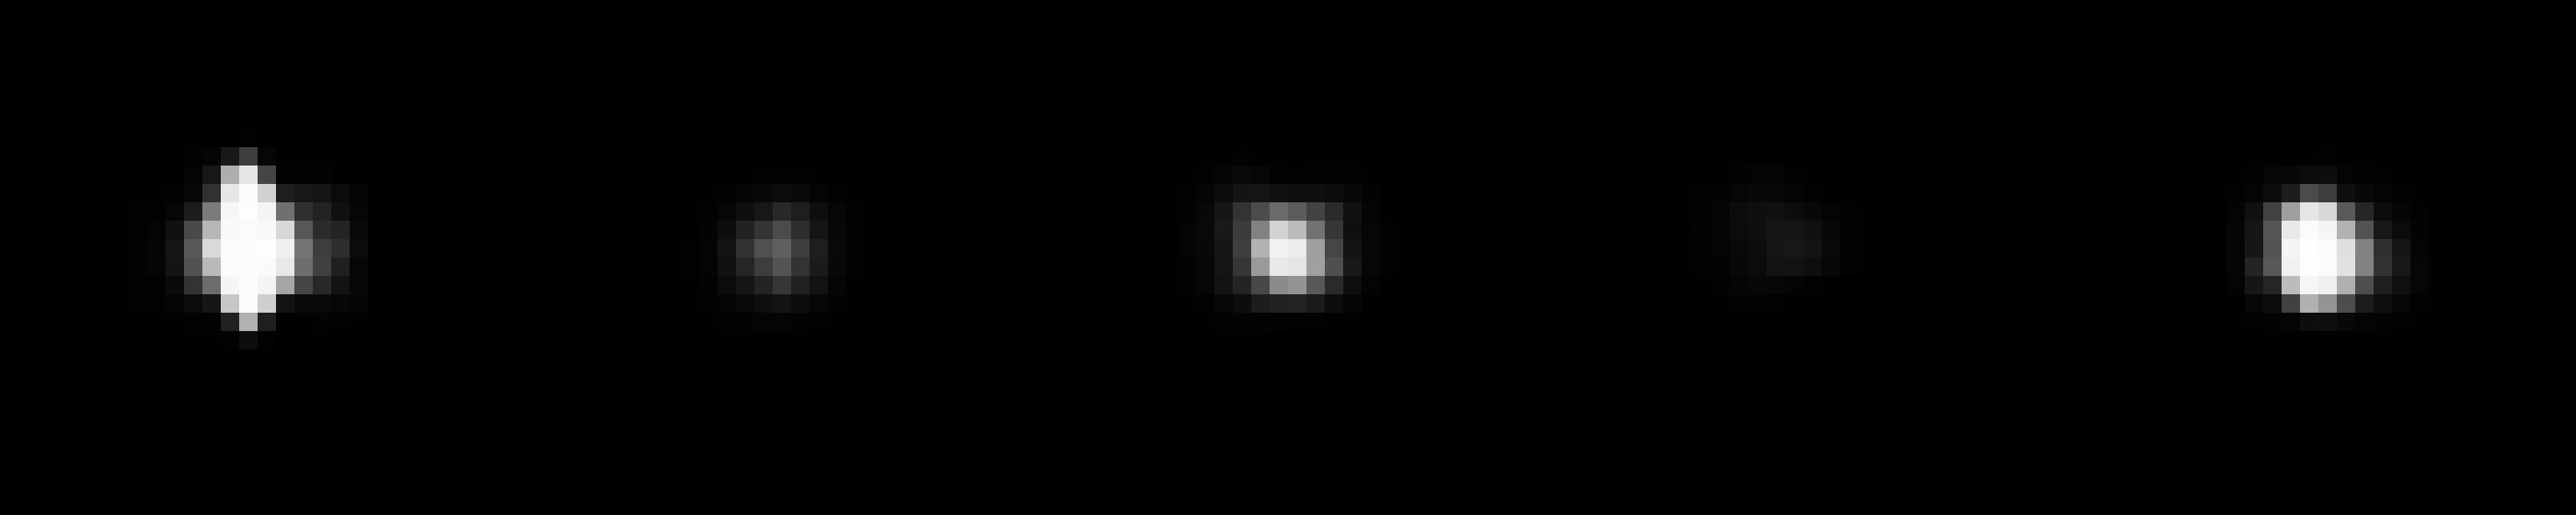
\includegraphics[width=\columnwidth]{assets/clustered_generated_stars_resized.png}
    \caption{Samples of the five different star classes generated by the cDCGAN.}
    \label{fig:clustered_generated_stars}
\end{figure}

\begin{figure}
    \centering
    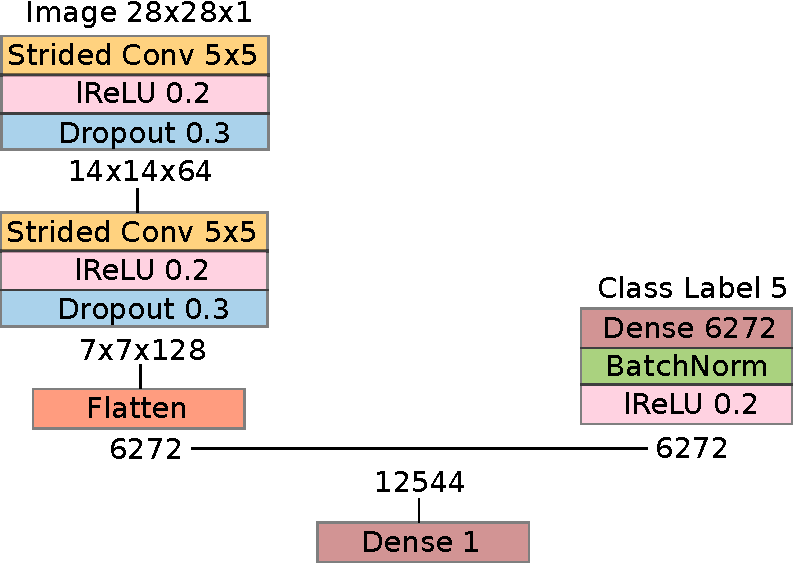
\includegraphics[width=0.73\columnwidth]{assets/cdis_arch.pdf}
    \caption{Illustration of the architecture of the conditional discriminator. The image of dimension $\SI{28}{}\times\SI{28}{}\times1$ is downsampled by two convolutional layers with stride \SI{2}{} and a $\SI{5}{}\times\SI{5}{}$ kernel (denoted by ``Strided Conv 5x5), flattend and then combined with class label latent code, which was mapped from dimension \SI{5}{} to \SI{6272}{} by a dense layer. ``Dense 1'' maps this combined latent code to a $1$-dimensional prediction between \SI{0}{} and \SI{1}{}.}
    \label{fig:cdis_arch}
\end{figure}







%\subsubsection{PixelCNN on stars}
%For the PixelCNN, we adopted the code from Gupta \cite{Gupta}, which follows the work from van den Oord et al.\@ \cite{PixelCNN}. We evaluated a conditional and an unconditional setting. The results looked strictly worse than those of the (c)DCGAN in both settings, so we did not bother to include the code any further into our existing project.

\section{Results}
\label{sec:results}

Table \ref{tab:RF} shows the results of our different random forest regression models (RF). By using histograms of different image properties, we were able to improve the accuracy of the regression as measured by the mean absolute error (MAE) by a factor of approximately 3 with respect to the baseline.

%The evaluation of our models for approximating the similarity function is pretty straightforward. All models were evaluated on Kaggle. The results are shown in Table \ref{tab:SFA_MSS}.
All of our models for approximating the similarity function were evaluated on Kaggle. The results are shown in Table \ref{tab:SFA_MSS}.
%During the training of the CNN, we also calculated the MAE of the model on the validation set that was kept separate from the training set. These results are visible in Table \ref{tab:SFA_MSS}. While the RF models were also initially trained on a training set and were validated locally with the rest of the data from the scored data set, the models used for the approximation of the query set were trained on the whole data set. 
%For the CNN, we additionally calculated the MAE on the local \SI{20}{\percent} validation split. Since the RF is not as prone to overfitting, the final model was trained on the whole set. As such, we do not have local scores for the RF models in Table \ref{tab:SFA_MSS}.
%We have also included training and scoring time for these models in Table \ref{tab:SFA_time}. We built all our neural networks with the Keras (Chollet et al.\@ \cite{chollet2015keras}) API using TensorFlow (Abadi et al.\@ \cite{tensorflow2015-whitepaper}) backend and trained them on the Leonhard cluster, using the NVIDIA Tesla V100-SXM2 \SI{32}{GB} GPU. One can clearly see that our best RF model outperforms the CNN in both score and performance time.
For the CNN, we additionally calculated the MAE on our local \SI{20}{\percent} validation split. Since the RF was prone to overfitting, it was trained without a local validation split and local results are omitted. We included training and scoring time for these models in Table \ref{tab:SFA_time}. 

%One can see that our best RF model outperforms the CNN baseline in both accuracy and performance.

%From the baseline RF model to our best RF model we were able to improve the accuracy of the regression as measured by the mean absolute error (MAE) by a factor of approximately 3. The results are shown in Table \ref{tab:RF}.

%We also included training and scoring time for all our similarity score models in Table \ref{tab:SFA_time}. One can clearly see that our best RF model outperforms the CNN in both accuracy and performance.

For our generative models, we decided to follow the evaluation process of the Kaggle competition and used our best RF model and the CNN to estimate the mean similarity score of the generated images. The results are displayed in Table \ref{tab:gen_MSS}. The time needed for training and the generation of $100$ images is shown in Table \ref{tab:gen_time}. 

As shown in Figure \ref{fig:dcgan_stars}, the large DCGAN did not manage to capture the shape of important features in detail. Table \ref{tab:gen_MSS} shows the estimated similarity scores for these cosmology images.

Figure \ref{fig:vae_interpolation} shows linear interpolations between vectors in the latent space of the variational autoencoder (VAE) to demonstrate that the model works well. Table \ref{tab:gen_MSS} shows the estimated similarity scores for the corresponding cosmology images.

%To evaluate our generators we used our two best similarity function approximators, i.e.\@ our best RF model and CNN, to calculate the mean similarity score of the images. We chose not to train and use a conventional classifier to evaluate the generated images, as the Kaggle competition states that the images will be scored according to their mean similarity to a prototypical cosmology image. As such we decided to use the same evaluation process. These results are visible in Table \ref{tab:gen_MSS}. The time needed for training and generating $100$ images each for the various models is displayed in Table \ref{tab:gen_time}. 

\begin{table}\centering
    \begin{tabular}{lrr|rr}
    \toprule
        Model           & MAE           & STD           &  MAE          &  MAE \\
                        & (loc.)        & (loc.)        & (pub.)        & (priv.) \\
    \midrule
        RF (baseline)   & -             & -             & \SI{0.258}{}  & \SI{0.287}{} \\
        CNN             & \SI{0.174}{}  & \SI{0.279}{}  & \SI{0.168}{}  & \SI{0.188}{} \\
        RF (best)       & -             & -             & \SI{0.095}{}  & \SI{0.105}{} \\
    \bottomrule
    \end{tabular}
\caption{Mean absolute error (MAE) and standard deviation of the absolute error (STD) of our models approximating the similarity function.}
\label{tab:SFA_MSS}
\end{table}

\begin{table}\centering
    \begin{tabular}{lrr|rr}
    \toprule
        Model           & RF MSS                & RF STD        & CNN MSS               & CNN STD \\
    \midrule
        AG (baseline)   & \SI{1.718}{}          & \SI{0.910}{}  & \SI{1.450}{}          & \SI{0.697}{} \\
        large DCGAN     & \SI{1.069}{}          & \SI{0.717}{}  & \SI{1.154}{}          & \SI{0.773}{} \\
        VAE             & \SI{1.690}{}          & \SI{0.555}{}  & \SI{2.031}{}          & \SI{0.662}{} \\
        cDCGAN          & \textbf{\SI{3.018}{}} & \SI{1.220}{}  & \textbf{\SI{2.746}{}} & \SI{1.048}{} \\
    \bottomrule
    \end{tabular}
\caption{Mean similarity score (MSS) and standard deviation of the similarity score (STD) of the images generated by our models as estimated by our CNN and best RF model.}
\label{tab:gen_MSS}
\end{table}

\begin{table}\centering
    \begin{tabular}{lrr}
    \toprule
        Approximator    & Training time     & Scoring time \\
    \midrule
        RF (all)        & \SI{1.5}{\hour}   & \SI{2}{\minute} \\
        CNN             & \SI{24}{\hour}    & \SI{1}{\minute}  \\
        %RF (best)       & \SI{1.5}{\hour}     & \SI{2}{\minute} \\
    \bottomrule
    \end{tabular}
\caption{Training and scoring time for our various similarity function approximators (including preprocessing).}\label{tab:SFA_time}
\end{table}

\begin{table}\centering
    \begin{tabular}{lrr}
    \toprule
        Generator   & Training time     & Generation time \\
    \midrule
        AG          & -                 & \SI{<1}{\minute} \\
        large DCGAN & \SI{2.5}{\hour}   & \SI{<1}{\minute} \\
        VAE         & \SI{2}{\minute}   & \SI{<1}{\minute} \\
        cDCGAN      & \SI{30}{\minute}  & \SI{<1}{\minute} \\
    \bottomrule
    \end{tabular}
\caption{Training and generation time for our various generators.}
\label{tab:gen_time}
\end{table}

\begin{table}\centering
    \begin{tabular}{lrrr}
    \toprule
        & \# features & MAE & MAE \\
        & & ~(pub.) & ~(priv.) \\
    \midrule
        Pixel intensity (baseline) & \SI{32}{} & \SI{0.258}{} & \SI{0.287}{}  \\
        Pixel intensity + oriented gradients & $\SI{32}{} + \SI{36}{}$ & \SI{0.183}{} & \SI{0.203}{} \\
        Power spectrum & \SI{48}{} & \SI{0.107}{} & \SI{0.124}{} \\
        Power spectrum + ROI & $\SI{48}{} + \SI{48}{}$ & \SI{0.095}{} & \SI{0.105}{} \\
    \bottomrule
    \end{tabular}
\caption{Mean absolute error (MAE) for random forest regression using different features.}
\label{tab:RF}
\end{table}

\section{Discussion}

From Table \ref{tab:SFA_MSS} we can observe that all of our models for approximating the similarity function outperform the baseline. Presently, classification is mostly dominated by CNNs. Still, our RF model performed significantly better than our CNN. We thus conclude that for sparse data of limited range, there are still methods beside neural networks that can be useful. 

Table \ref{tab:gen_MSS} shows that the cDCGAN achieves the highest mean similarity score (MSS) of all models and also significantly outperforms the baseline in terms of MSS. Besides the highest MSS, the cDCGAN also reaches the highest standard deviation (STD). This is because we try to approximate the star distribution with ``good'' random numbers by choosing those giving the highest MSS. An additional neural network could have learnt to produce the ``perfect'' set of cosmology images by learning the star distribution on its own. %newline or no newline here?

The large DCGAN does not exceed the performance of the baseline and is outperformed by both VAE and cDCGAN. This shows that we were indeed able to improve our results by focusing on the generation of key features only.


%Besides the highest mean similarity score (MSS), the cDCGAN also reaches the highest standard deviation (STD). This is because we try to approximate the star distribution with ``good'' random numbers by choosing those giving the highest MSS. Instead, an additional neural network could have learnt to produce the ``perfect'' set of cosmology images by learning the star distribution on its own. The trained CNN regression model could have been used as a loss function. However, because of gradient computations, the RF model could not have been used. 



%This is due to the fact that the images are very sparse and the range of images is very small, i.e.\@ they all mostly look the same (beside the ones that are definitely not cosmology images). In general, an algorithm that scores an image according to its histograms will not be able to achieve as high an accuracy as a well-built neural network. 

\section{Summary}

By extracting the most important features from our cosmology images and by designing generative models for only these, we were able to obtain highly realistic results.

%By selectively extracting the most important features from our cosmology images and learning to generate only these, we achieved generated images superior to whole generated images.
%than if the generative model learns to generate the image as a whole. \TODO{"superior than if" sounds strange, should probably be something with "superior to"...}
%This is judged by our similarity scorers.

For the approximation of the similarity function, we found that our cosmology images are best characterized by their power spectrum. Lastly, despite being more complex, a CNN does not always necessarily outperform a simpler model such as random forest. % deleted "a"

%For the similarity scorers of cosmology images, we have found that preprocessing in the form of the power spectrum and the use of ROI histograms improved the approximation by a significant amount. Lastly, despite being more complex, a CNN does not always necessarily outperform a simpler model such as a RF.

\section*{Acknowledgements}
We would like to thank the assistants of the Computational Intelligence Lab for all their support and invariably fast replies to all our questions.

\newpage


\bibliographystyle{IEEEtran}
\bibliography{cil_report}

\clearpage

\includepdf{assets/CIL_declaration_originality_Till.pdf}

\includepdf{assets/CIL_declaration_originality_Sven.pdf}

\includepdf{assets/CIL_declaration_originality_Michelle.PDF}
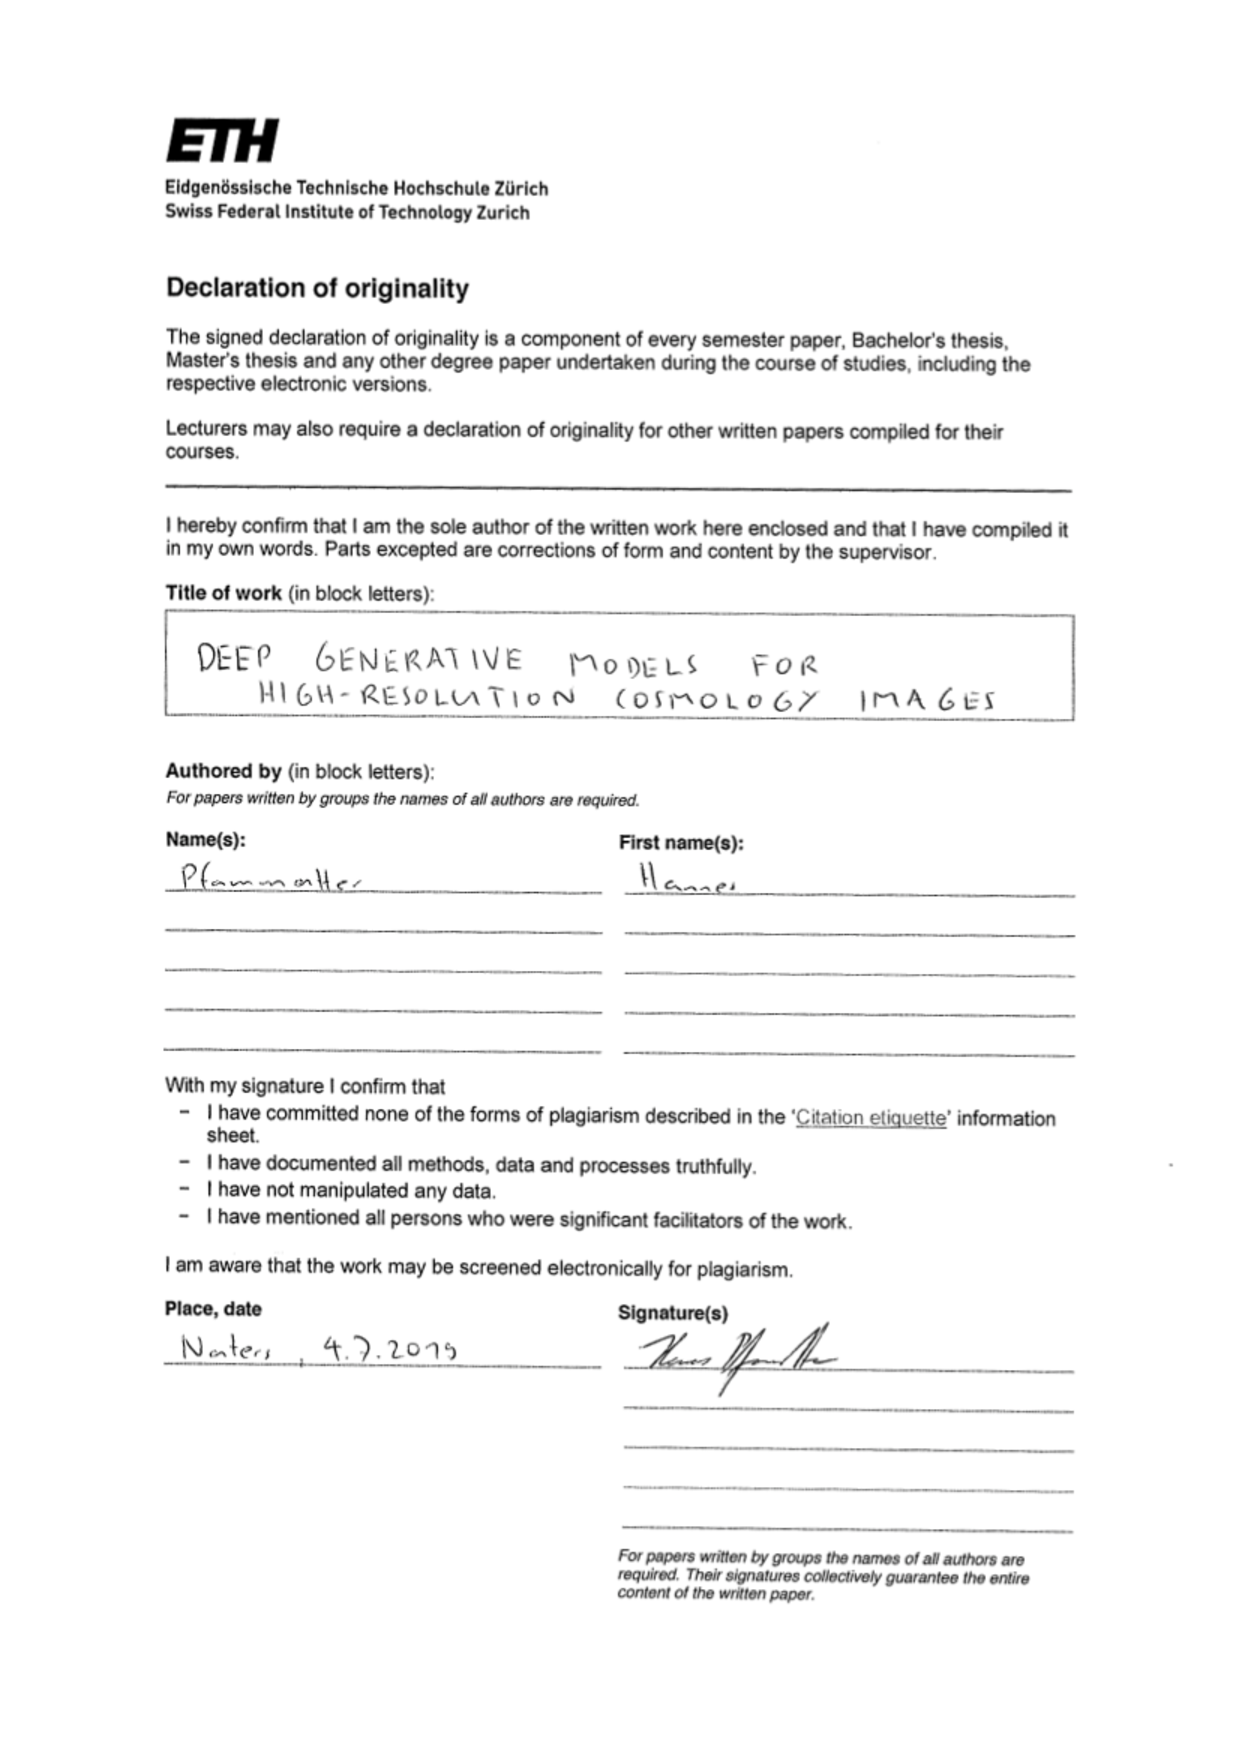
\includepdf{assets/CIL_declaration_originality_Hannes.pdf}

\end{document}
